\section{Web}

The software in the \texttt{web/} folder is a svelte web application that allows the user to connect to PiRover, view the live camera feed and control the Rover. An image follows:

\begin{figure}[H]
    \centering
    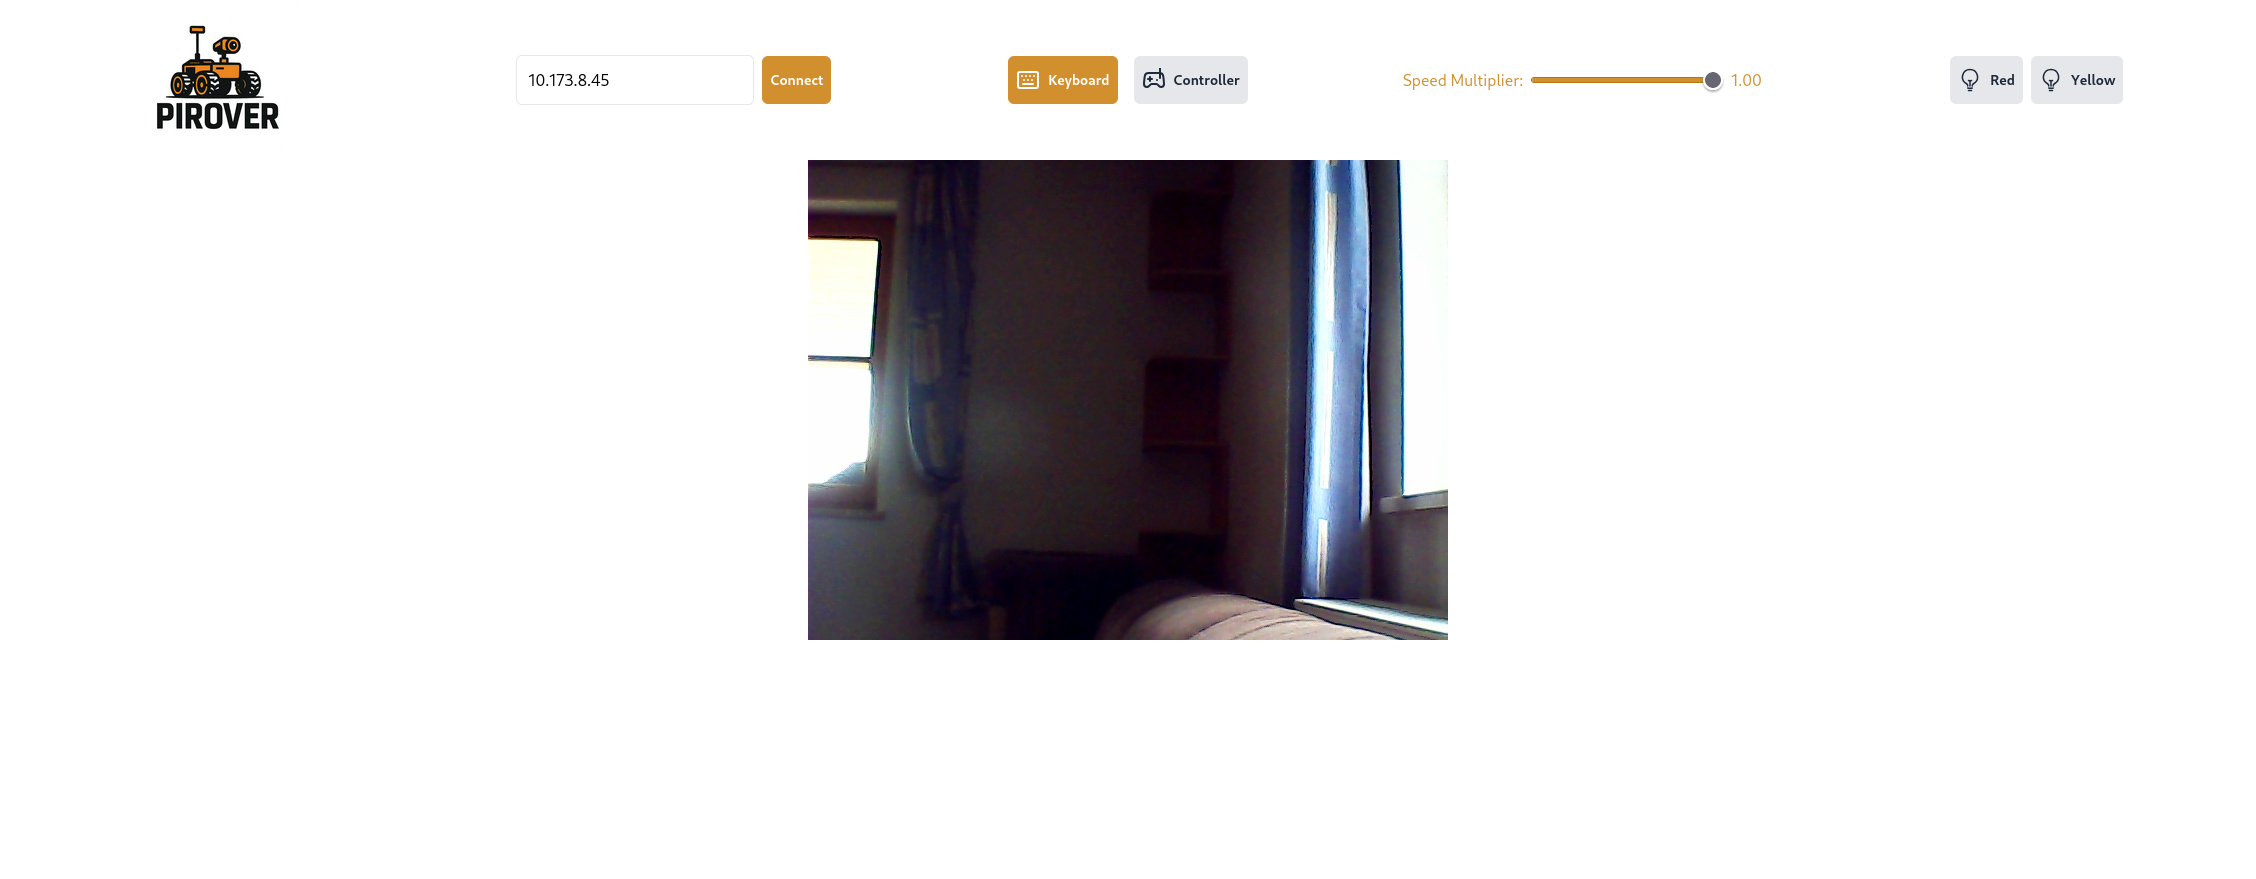
\includegraphics[width=\textwidth]{img/web.png}
\end{figure}

The following controls are available:

\begin{itemize}
    \item driving forwards and backwards
    \item steering the front wheels
    \item making the camera look in a different direction
    \item activating and deactivating the buzzer
    \item activating and deactivating either a red or an orange light
\end{itemize}

The application connects to PiRover via websockets. Tailwind CSS is used to make styling more elegant. In the following, we will examine the critical files and functionalities in more detail, file by file:

\subsection*{\texttt{App.svelte}}

This is the main Svelte component that holds the web application together. It defines an input where you can enter an IP address to connect to PiRover. It also specifies the creation of the websocket connection. Once connected, this file also displays controls for switching between keyboard and gamepad as the input method, buttons to turn PiRover's lights on and off, a slider that can make PiRover go faster or slower and the live camera feed. It also defines the handler functions to send the various controls to PiRover via the websocket connection. To make the application more modular, however, we extracted the functionality to display the live camera feed and to detect inputs into the separate Svelte components \texttt{Camera.svelte} and \texttt{Controls.svelte}.

\subsection*{\texttt{Camera.svelte}}

This file listens to the websocket connection and displays the image if available.

\subsection*{\texttt{Controls.svelte}}

This component primarily defines the buttons to switch between keyboard and gamepad as the input method. These buttons internally either set an instance of the \texttt{keyboard.ts} class or an instance of the \texttt{gamepad.ts} class as the current source. These classes both implement the \texttt{source.ts} interface to make this more elegant. The inputs received from the current source then basically get forwarded to the websocket connection and sent to PiRover. 

\subsection*{\texttt{source.ts}}

On the one hand, this interface defines a field \texttt{state} that describes the current state of the input method, like the current camera direction or steering angle. On the other hand, it defines what actions an implementation of the \texttt{Source} interface should notify us about. The implementations \texttt{keyboard.ts} and \texttt{gamepad.ts}  then simply modify the state field and notify us about the interesting inputs according to the specifics of the respective input method.

